\chapter{绪论}

% 社会的发展和经济的进步,导致人们的生活节奏越来越快。高强度的工作以及不健康的生活方式让处于亚健康状态的人们越来越多,健康养生也愈发成为当前热门的话题。同时,有限及分配不平衡的医疗资源经常不能及时地满足广大群众健康管理的需求\cite{雷鹏2019中国医疗资源配置与服务利用现状评价}。
% 信息技术,尤其是日常健康管理技术是解决这一问题的重要途径。健康管理技术可通过采集用户的心率,体重,血压等信息(通常需要借助额外的传感器等设备完成数据的采集),帮助用户了解自身的健康状况。
% 在这些可获取的信息中,面部信息除了用于识别身份、情绪之外,也包含大量和健康相关的信息。通过面部信息大致判断个人身体状况的面诊技术也有充足的理论与技术基础\cite{li2020tcminet}。
% 随着面诊技术相关研究的不断深入,基于面诊技术的各类健康管理系统也在探索中\cite{林锋2019中医面诊系统调研报告}。

% 现有的研究大多局限于医疗环境,面向日常健康管理的面诊系统如何设计却缺乏对应的研究,各类面诊系统的设计也存在各种局限性。
% 面向专业医疗环境开发出来的面诊系统是否可以直接应用于日常健康管理?面向日常健康场景的面诊系统可能存在哪些问题?
% 面向日常健康场景的面诊系统可以遵循哪些设计策略?在设计系统时如何保证系统的通用性和可拓展性?
% 研究这一系列问题,将有助于面诊技术应用到日常健康场景中,满足用户日常健康管理的需要。

\section{研究背景及意义}
% 亚健康与慢性病问题严重, 医疗资源不足
健康问题是当前社会不可忽视的问题:一方面,随着经济建设的步伐加快,我国处于亚健康状态的人群愈发庞大,在白领阶层更加严重\cite{health_report2019};
% 亚健康通常用于描述一个人心理或生理处于健康与疾病的中间状态,虽然短期以来不影响人的正常生活,但会长期影响人的生活质量。
% 根据上海外服健康管理中心的30万份体检数据,2014年到2018年间上海的亚健康指数已经从94.6\%上升到98.7\%,同时健康意识指数也从82\%上升到84\%\cite{health_report2019}。
另一方面,当前人们享受着比以往时代更加长寿的生活,寿命的增加也间接造成了慢性病患病率的提高\cite{OlshanskyDEMOGRAPHY}。
慢性病如糖尿病、高血压等,作为一种长期的疾病,大多数在目前的医疗条件下是无法治愈的,会伴随患者一生,也越来越得到人们的重视\cite{blandford2019hci, lupton2017self-tracking}。

为了解决亚健康与慢性病给用户的生活带来的相关问题,人机交互的相关研究中如何有效支持日常健康管理成为了一个热门的研究课题。
从研究出发点看,人机交互中的日常健康管理可分为慢性疾病管理和鼓励用户形成健康的生活方式两大类,主要实现方案是通过合理的系统设计,对各类健康相关指标的监测,让慢性病患者可以在日常生活中有效管理慢性病,从而更加健康地生活。
但目前这些健康追踪和监测技术,主要的实现方式还是通过量化采集用户的健康指标相关的数据,并没有考虑到利用面部信息。
% 近年来,人机交互领域中的关于日常健康管理的研究包括增强用户的日常生活体验、加强患者与医护人员的沟通和协作、提高用户的疾病认知等方面。
% 在有限的医疗资源以及经济条件的背景下,慢性病患者不会一直待在医院,需要日常长期坚持服药或保持特定的饮食生活习惯,对原来的正常生活造成诸多影响\cite{lupton2017self-tracking}。

% 日常健康管理的重要性。
% 人机交互(Human-Computer Interaction/ HCI)是研究计算机技术应该如何设计使其更好的为人服务的跨学科领域。为了解决亚健康与慢性病给用户的生活带来的相关问题,人机交互的相关研究中如何有效支持面向日常健康的自我管理成为了一个热门的研究课题。
% 近年来,人机交互领域中的关于日常健康管理的研究包括增强用户的日常生活体验、加强患者与医护人员的沟通和协作、提高用户的疾病认知等方面。
% 从研究出发点看,人机交互中的日常健康管理可分为慢性疾病管理和鼓励用户形成健康的生活方式两大类,主要实现方案是通过合理的系统设计、对各类健康相关指标的监测,让慢性病患者可以在日常生活中有效管理慢性病,从而更加健康地生活。其中,对用户健康相关指标监测可以大致分为两大类:
% \begin{enumerate}
%     \item 日常行为的监测:通过监测用户的日常饮食、运动情况等日常行为,培养用户更好的饮食习惯、锻炼习惯等\cite{purpura2011fit4life,Inagawa2013A,cordeiro2015barriers, miller2014stepstream}。例如Yuma Inagawa等\cite{Inagawa2013A}开发了一个营养管理和检索系统,根据用户的喜好给出推荐的菜单,用户也可以给出对应的反馈,以此来培养用户健康的健康饮食的观念,进而达到引导用户形成更健康的饮食习惯的目的。
%     \item 健康指标的监测:健康指标主要包括生命体征如呼吸、血压、心率,也包括睡眠、体重等以帮助用户及时了解自己的健康状况,进行及时的干预和调整\cite{kay2012lullaby,gronvall2013beyond,walters2010a}。
% \end{enumerate}

% 这些日常健康管理技术,在有效改善与控制慢性病方面起着至关重要的作用\cite{ayobi2017quantifying}。
% 但目前这些健康追踪和监测技术,主要的实现方式还是通过量化采集用户的健康指标相关的数据,并没有考虑到利用面部信息。

% 近年来,随着面部识别技术的迅速发展,也有越来越多通过采集面部信息获得健康相关数据的研究。

% 面部信息有丰富的健康相关特征,也有丰富的面部信息和健康相关的理论研究。大量研究表明,面部是反映一个人身体健康和精神面貌的重要部位,能够透露出各种健康状况甚至体内疾病的迹象。
% 在现代医学领域,当医生评估患者的总体体质并得出可能疾病的初步假设时,直接观察面部是医学诊断的一部分\cite{ding2019reading}。
% 内部器官的病变会导致面部出现对应的症状,通过观察面部对应的症状,如面部的颜色、形状、斑点等,可以大致推测内部器官的情况\cite{汪珺2018六经辨证中自然辩证法三大规律初探}。
% 此外,医疗领域不仅有经验充足的面诊理论基础,大量学者也为面诊信息化做了实证研究,如面色和乙肝关系的研究\cite{吴秀艳2014108}、基于舌部特征判断慢性肾衰竭\cite{周小芳2018慢性肾衰患者虚兼湿浊证的口唇特征研究}等。
% 此外,面诊在中国有深厚文化基础。面诊作为传统中医四诊(望闻问切)中重要的一步,在中国有深远的影响,大部分人都接受或理解通过观察面部进行健康诊断的方式。

% 技术基础, 介绍面诊系统的基本原理和发展

面部信息有丰富的健康相关特征\cite{ding2019reading},也有丰富的面部信息和健康相关的理论研究,如面色和乙肝关系的研究\cite{吴秀艳2014108}、基于舌部特征判断慢性肾衰竭\cite{周小芳2018慢性肾衰患者虚兼湿浊证的口唇特征研究}等。随着人工智能特别是基于深度学习的计算机视觉技术\cite{hassaballah2020deep}的发展,面诊技术变得日益成熟和广泛,将计算机面诊技术引入到日常健康场景下在技术上变的可行,在中国大部分人也接受面诊这一诊断方式。
面诊技术,主要通过用户的面部信息、舌部信息等作为输入,通过预处理、面部兴趣区域提取、特征提取、特征分类、规则系统等方法,最终得到用户的健康相关信息,如体质倾向,健康分数等\cite{林锋2019中医面诊系统调研报告}。
相比当前的基于穿戴式和便携式设备的日常健康诊断方法,在移动设备上基于面诊技术的日常健康管理有明显的优势:(1)不需要额外的设备。当前的移动设备可以方便地获取用户的面部信息,基于面诊技术的日常健康管理应用成本更低,日常使用也更加方便。(2)大部分人在日常生活中有使用手机自拍的习惯,面诊也有悠久的文化基础和扎实的理论基础,基于面诊技术的日常健康管理可以融入到日常健康场景中。

人机交互是一个研究技术怎么使用和设计的学科,其中一个重要的共识是上下文与场景对我们的日常行为和技术使用起到关键性作用:当场景发生变化之后,对于技术怎么使用和怎么设计存在关键性影响\cite{1987Plans}。
目前已有的基于面诊技术的面诊系统主要是面向诊所医院等专业环境,相关研究也都集中在面诊算法上,现有研究缺乏对日常场景下用户会如何使用面诊技术以及面诊系统应该如何设计这方面的理解。
虽然在面诊技术在算法研究部分其准确性在不断提高,但在如何基于面诊技术设计面诊系统、将面诊技术集成到日常健康管理的场景中,目前相关的工作还极其匮乏。
研究面诊系统在日常健康管理场景下的应用问题,需要通过实地调研,分析面诊技术在日常健康场景下的特点,了解用户的需要以及遇到的问题,帮助用户更好地使用面诊系统。
深入研究日常健康场景下的面诊系统设计与实现,将有助于将面诊技术从专业的诊所环境应用到日常健康场景,辅助用户进行日常健康管理,从而在一定程度上缓解当前整体公共医疗资源不足的压力,改善用户的生活品质。

\section{研究现状与挑战}
本文关注日常健康场景下的面诊系统设计与实现,因此研究现状将分面诊系统与人机交互领域中的日常健康管理研究两部分介绍。
% 一方面,面诊技术的出现和发展为支持日常健康场景下的健康管理提供了新的解决方案,但目前主要探索还是在算法的探索上,而系统设计也是主要针对标准的诊所环境,针对日常健康管理场景的研究还比较少。
% 另一方面,人机交互虽然有大量关于日常健康场景下的系统设计工作,但目前也集中在慢性病管理和健康行为引导等方面,并未考虑到利用面部信息进行健康诊断的系统设计。
% 目前关于日常健康场景下的面诊系统设计还极其匮乏。

\subsection{面诊系统}
\label{subsec:面诊系统}
面诊技术是面诊系统的基础,为了能够设计符合日常健康管理场景下的面诊系统以及帮助读者理解设计面诊系统的难点,本小节将先介绍面诊技术的特点,然后再介绍当前常见的面诊系统设计。
% \subsubsection{面诊技术简介与特点}

本文对以往面诊技术中所用算法以及面诊系统相关的文献和技术进行了调研与分析。
% 面诊算法,作为面诊技术的重要部分,其输入主要为用户的面部信息,同时也可能包括舌部信息,或者其他相关特征,最终得出用户的健康相关信息,如健康程度、体质分类、疾病倾向等。
% 起初,面诊技术主要研究点在如何基于信息化技术辅助医护人员获取用户相关特征,涉及到的算法有面部信息采集、人脸检测、面部区域分割、图像标准化、色彩矫正、面部特征提取等\cite{宋海贝2018中医面诊信息自动识别方法研究进展},
% 其中人脸检测、面部区域分割、图像标准化、色彩矫正为预处理方法,可以为后续面部特征提取提供基础数据。
% 随着研究的深入,相关研究在探索面部信息与疾病的关联关系的同时也在尝试通过算法来代替专业医生判断健康状况,如各种分类模型如基于规则的分类器、SVM(Support Vector Machine)分类器、深度学习模型等\cite{林锋2019中医面诊系统调研报告}。
总的来说,面诊技术有以下特点:(1)涉及的算法数量多如面部信息采集、人脸检测、面部区域分割、图像标准化、色彩矫正、面部特征提取等\cite{宋海贝2018中医面诊信息自动识别方法研究进展},且随着技术的快速发展,算法更新迭代频率高\cite{esteva2021deep}。(2)不同的算法和算法之间有依赖关系。如唇部区域提取算法,通常需要面部图片进行人脸识别,得到分割之后的面部图片作为输入\cite{Hu2016Robust}。(3)面诊的流程长且复杂\cite{林锋2019中医面诊系统调研报告}。
面诊系统随着面诊技术的发展主要分以下几类。

\begin{figure}[h]
    \centering
    \subfigure[面诊仪\cite{邸丹2016手持式舌象仪的研制}]{
        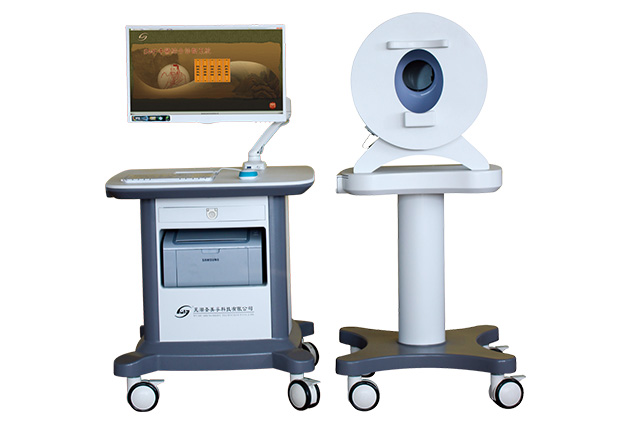
\includegraphics[width=4.5cm]{images/SMF.jpg}
    }
    \subfigure[日常场景下的智能诊断设备\cite{andreu2015mirror}]{
        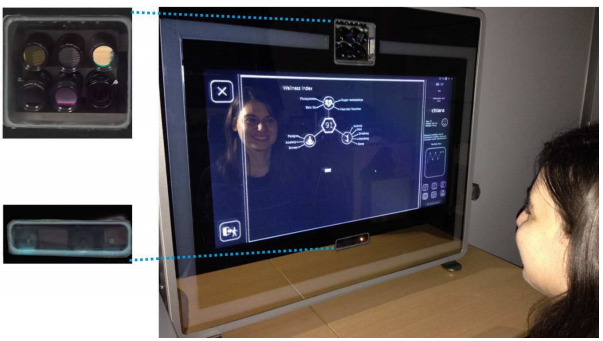
\includegraphics[width=4.5cm]{images/mirror.png}
    }
    \subfigure[移动平台上的面诊应用\protect\footnote{www.huihujiankang.cn}]{
        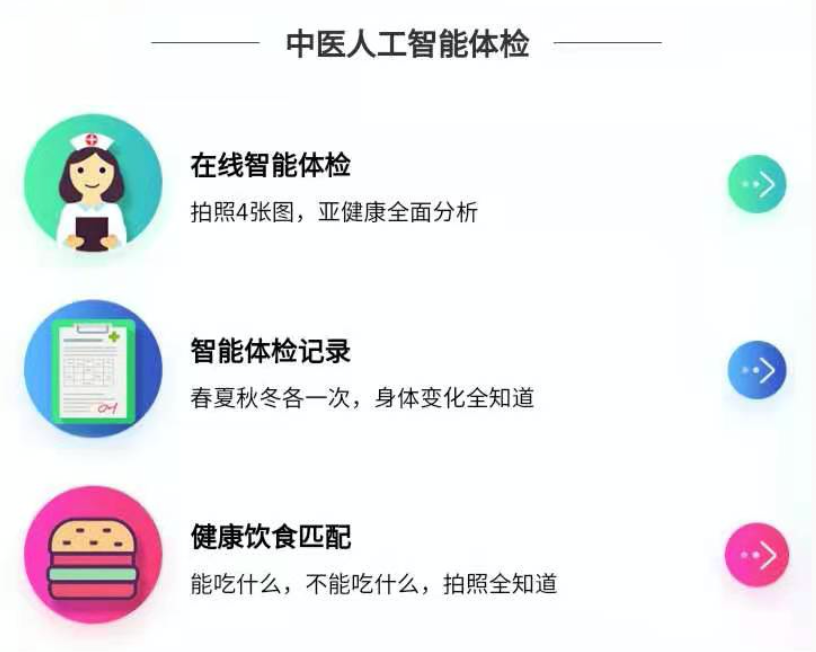
\includegraphics[width=4.5cm]{images/apps.png}
    }
    \caption{当前的一些面诊系统}
    \label{fig:med}
\end{figure}

在面诊技术相对成熟的基础上,以面诊仪为代表面诊系统主要目的是提高传统面诊效率,辅助医护人员\cite{邸丹2016手持式舌象仪的研制, 李丹溪2017舌诊仪的发展及其在舌诊客观化研究中的应用现状}。
以往的面诊需要专业的医生观察患者的面部,结合各方面患者的综合情况,根据中医面诊理论得出最终的诊断结果。
传统面诊模式制约了中医的现代化推进,一方面,传统的面诊方式存在以下明显的缺点:效率低,需要专业医生参与,且易受到医生对患者身体状况主观判断的影响。
面诊仪是为诊所环境研发的一类面诊系统,其主要目的是为了减轻医生的负担,同时在一定程度上将诊断依据客观化,避免人为的主观判断导致结果出现偏差\cite{李丹溪2017舌诊仪的发展及其在舌诊客观化研究中的应用现状}。
随着诊断理论客观化研究的进一步深入,面诊系统开始关注自动分析诊断能力,辅助医护人员进行临床诊断。

早期的面诊仪可作为初步信息采集工具得到患者的面色、舌象等信息,但随着诊断理论客观化研究的发展,也有相关工作在面诊仪的基础上提供了一定的自动化分析诊断能力,如面色自动识别分析系统\cite{崔骥2018人工智能背景下中医诊疗技术的应用与展望}。
诊断理论客观化研究即使用计算机信息化技术,通过理论研究与实验研究,将传统与临床的诊断理论,系统地研究出其量化的本质,包括量化面色、舌象、脉搏信息与健康指标的关系,从而为其信息化应用提供基础\cite{Wang2013TCM, guo2015analysis, li2020tcminet}。
在临床上,也有大量利用信息化技术进行关于面部信息与冠心病、慢性肾衰竭、脑血管病等相关分析,从而为诊断提供相应的辅助功能\cite{崔骥2018人工智能背景下中医诊疗技术的应用与展望}。
除面诊仪外,在中医面诊标准化、客观化、信息化的基础上,不少基于中医面诊理论的面诊系统也随之出现。
常见的基于中医的面诊管理系统,其设计的初衷是在诊所的标准环境下服务于医护人员,如中医望诊装置\cite{李国正0一种用于中医望诊的三维图像采集装置}和中医面诊分析诊断系统等\cite{李福凤2016中医面诊分析与诊断系统}。
这类系统功能比较单一,主要是帮助医护人员采集数据以及辅助诊断,在使用上对精度要求相对高,需要专业人员经过培训在标准环境下操作,在日常场景下很难实现这些要求。

随着医疗智能的发展,市面上开始出现各类面诊智能医疗设备,如智能诊断机器人\footnote{www.huihujiankang.cn}、家用面诊仪等,
同时如图\ref{fig:med}-(3)所示移动平台上也出现了大量的面诊应用如慧虎面诊应用\footnote{www.huihujiankang.cn/s-33.html}, 寻艾AI\footnote{www.xun-ai.cn}等,这类面诊系统降低了对设备和诊断准确率的要求,主要辅助用户判断自己大致的身体情况。
但因为沿用了诊所环境下的设计,鉴于诊所环境与日常健康场景的显著性差异,这些面诊系统实际能否直接适用于日常健康场景还是未知的。
% 在诊所环境下,医院能够承担昂贵的设备费用,能提供标准的拍摄环境,并且全程有对医护人员规范的操作流程的培训;在日常健康场景下,用户的文化水平、拍摄环境存在差异,并且需要考虑到长期使用的情况。
复旦大学的林锋\cite{林锋2019中医面诊系统调研报告}等在中医面诊系统调研报告中提到:\myfont{不够便携、依赖医护人员、缺乏友好的人机交互这些问题,影响了面诊仪从医疗环境迁移到日常健康场景}。
成都中医药大学的宋海贝\cite{宋海贝2019中医面诊健康管理系统}等在中医面诊健康管理系统的专利中也提到:\myfont{虽然目前有大量成功应用的面诊智能医疗设备,但它们并不适用于日常使用}。
因此宋海贝等以日常健康管理的面诊系统的角度出发,利用智能镜子、智能终端、云端处理器等模块,实现了日常健康场景下的一个中医面诊健康管理系统。
该研究基于日常健康管理这一场景的特殊性进行系统设计,但只考虑到了长期使用的问题,在其工作中并未看到深入的日常场景的用户研究,对面诊技术在日常场景的理解还不够充分。

类似的,国外也有类似地考虑日常健康场景下面诊系统的系统设计。如图\ref{fig:med}-(b)所示,SEMEOTICONS\cite{andreu2015mirror}是一款放在家庭室内环境的镜子,通过摄像头和传感器采集面部信息和体温,监测与心血管疾病相关的疲劳、压力和焦虑等特征,让用户能够监测自己的健康情况,并根据量身定制的健康指南来改善用户的生活方式。
该系统由室内的硬件设备和远程服务器一起完成健康监测的功能,室内设备负责采集数据,远程服务器负责处理数据分析结果。
在生活中照镜子属于日常行为,该研究将面诊技术和日常行为结合起来,并且将应用场景拓展到了日常健康场景。
他们后续还进行了一次用户体验研究,研究结果表明\cite{coppini2017user}他们的原型系统的设计被大多数用户所接受:虽然测试过程非常耗时,大多数参与研究中的志愿者仍然很愿意完成并按计划进行实验,部分志愿者考虑了系统给出的健康指南,甚至因此改变了自己的生活方式。
总的来说,该系统通过将诊断和日常的照镜子的行为结合起来,可以很方便与用户的日常生活融合起来,同时在服务器端也可以方便的实现算法模型的适配和更新。
SEMEOTICONS的系统设计与其他面诊系统区别点在于系统设计的出发点就是考虑到日常健康环境,而不是基于现有诊所环境下的面诊系统迁移到日常健康环境,同时对原型系统进行了用户调研。
但是该系统固定在房间的某个位置使用的方式不够便携,同时该系统需要一系列的传感器设备,不仅增加了硬件的成本,部署起来也相对麻烦。


% 介绍发展背景,面诊算法发展,阐述当前的技术发展
% 以往的面诊需要专业的医生观察患者的面部,结合各方面患者的综合情况,根据中医面诊理论得出最终的诊断结果。
% 传统面诊模式制约了中医的现代化推进,一方面,传统的面诊方式存在以下明显的缺点:(1) 效率低,需要专业医生参与。(2) 对医生的要求比较高,且易受到医生对患者身体状况主观判断的影响,结果可能不够客观;另一方面,随着中医信息化的推进,各诊所对标准化用户信息采集、电子病历等要求也越来越迫切,因此推动了传统面诊方式进行改革。
% 而在计算机领域,与面部信息相关的读脸技术也在快速发展,这为面诊系统提供了技术基础。读脸技术(Face Reading Technology)通过读取人的面部图片获取相关的信息,主要应用有人脸检测、人脸识别、情绪识别、性别识别、年龄识别等\cite{Schroff2015FaceNet, Zhang2016Joint, corneanu2016survey}。
% % 基于面部图像分析的读脸技术在各领域的应用也越来越广泛如安全访问控制\cite{liu2005ibotguard}、身份识别\cite{he2015delving}、考勤管理\cite{surekha2017attendance}等。
% % 其中,读脸技术医疗环境中应用也成为研究热点,如基于读脸技术获取定位面部区域、获取面色舌苔唇色等,这类技术在标准环境配合在对应硬件采集设备如光电血流容积仪,色差仪等,已经可以达到足够的精度。
% 面诊仪\cite{邸丹2016手持式舌象仪的研制}是基于以上读脸技术研发的一类面诊系统,面诊仪其主要目的是为了减轻医生的负担,同时在一定程度上将诊断依据客观化,避免人为的主观判断导致结果出现偏差\cite{李丹溪2017舌诊仪的发展及其在舌诊客观化研究中的应用现状}。
% % 如道生面诊仪\cite{邸丹2016手持式舌象仪的研制}是目前某些医院用来采集面部信息的设备,芜湖圣美孚科技有限公司\footnote{http://www.smfkj.com/}也有一款舌面诊一体化设备。
% % 这类系统利用色差仪、可以实现面部图像采集以及面部特征提取,如面色、唇色、舌苔、舌象等,为诊断提供依据。

% \begin{figure}[h]
%     \centering
%     \subfigure[面诊仪]{
%         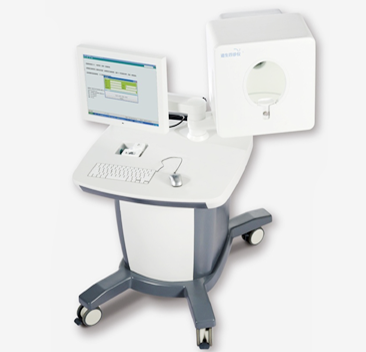
\includegraphics[width=5cm]{images/mzy.png}
%     }
%     \subfigure[舌面诊一体化设备]{
%         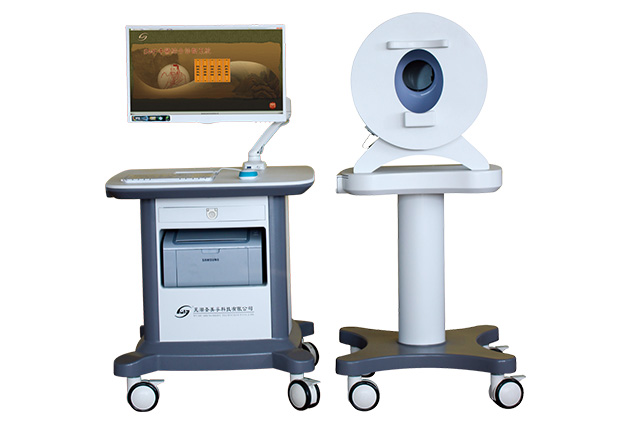
\includegraphics[width=5cm]{images/SMF.jpg}
%     }
%     \caption{面诊仪\cite{邸丹2016手持式舌象仪的研制}}
%     \label{fig:med}
% \end{figure}
% 介绍 面诊技术信息化 
% 早期的面诊仪可作为初步信息采集工具得到患者的面色、舌象等信息,但随着诊断理论客观化研究的发展,也有相关工作在面诊仪的基础上提供了一定的自动化分析诊断能力。
% 诊断理论客观化研究即使用计算机信息化技术,通过理论研究与实验研究,将传统与临床的诊断理论,系统地研究出其量化的本质,包括量化面色、舌象、脉搏信息与健康指标的关系\cite{Wang2013TCM, guo2015analysis, li2020tcminet},从而为其信息化应用提供基础。
% 在临床上,也有大量利用信息化技术进行关于面部信息与冠心病、慢性肾衰竭、脑血管病等相关分析,从而为诊断提供相应的辅助功能,如面色自动识别分析系统\cite{崔骥2018人工智能背景下中医诊疗技术的应用与展望}。
% % 则能得出初步的诊断结果,然后由医生再根据这些信息得到最终结果,在一定程度上减少了医生工作的负担。
% 除面诊仪外,在中医面诊标准化、客观化、信息化的基础上,不少基于中医面诊理论的面诊系统也随之出现。
% 常见的基于中医的面诊管理系统,其设计的初衷是在诊所的标准环境下服务于医护人员,如中医望诊装置\cite{李国正0一种用于中医望诊的三维图像采集装置}和中医面诊分析诊断系统等\cite{李福凤2016中医面诊分析与诊断系统}。

% 上海中医药大学的李福凤等基于中医望诊装置\cite{李国正0一种用于中医望诊的三维图像采集装置}的基础上,
% 利用模式识别相关算法,通过面部分割,面色、光泽、口唇特征分析等方法,实现了一个中医面诊分析与诊断系统\cite{李福凤2016中医面诊分析与诊断系统}。
% 该系统能够利用采集到的面部数据,对接医院的相关系统,自动为病人建立对应的电子病历,并给出一定的分析结果。
% 在分析结果的基础上,结合医生的专业诊断得到最终的结果,整体来说简化了面诊的流程,从而达到辅助医生临床诊断的效果。

% 随着低成本、高性能的移动设备出现,同时考虑到日常健康管理的越来越得到人们的重视,特别是在国外Self-tracking\cite{sanches2019hci}成为热门的研究话题,出现了大量关于日常健康管理的研究,
% 如在日常健康场景中通过移动设备监测口腔健康\cite{liang2020oralcam}、监测饮食\cite{burgermaster2019personal}等。
% 日常健康管理在慢性病管理、健康行为引导等方面也起到至关重要的作用,将面诊系统应用到日常健康场景具有重大的应用场景。


%这些研究虽然意识到日常健康场景与诊所环境的不同之处,但没有系统地使用人机交互的研究方法进行详细的用户行为分析,除长期数据这一方面外,日常健康场景下需要考虑的事情可能还有很多,很多细节需要进一步讨论。

% 类似的,国外也有类似地考虑日常健康场景下面诊系统的系统设计。Yasmina Andreu-Cabedo等\cite{andreu2015mirror}开发了SEMEOTICONS系统。
% SEMEOTICONS的系统设计与其他面诊系统区别点在于系统设计的出发点就是考虑到日常健康环境,而不是基于现有诊所环境下的面诊系统迁移到日常健康环境,同时对原型系统进行了用户调研。
% SEMEOTICONS是一款放在家庭室内环境的镜子,通过摄像头和传感器采集面部信息和体温,监测与心血管疾病相关的疲劳、压力和焦虑等特征,让用户能够监测自己的健康情况,并根据量身定制的健康指南来改善用户的生活方式。
% 该系统由室内的硬件设备和远程服务器一起完成健康监测的功能,室内设备负责采集数据,远程服务器负责处理数据分析结果。
% 在生活中照镜子本来就是每个人的日常行为,该研究将面诊技术和健康管理结合起来,并且将应用场景拓展到了日常健康场景。
% 他们后续还进行了一次用户体验研究,研究结果表明\cite{coppini2017user}他们的原型系统的设计被大多数用户所接受: 虽然测试过程非常耗时,大多数参与研究中的志愿者仍然很愿意完成并按计划进行实验,部分志愿者考虑了系统给出的健康指南,甚至因此改变了自己的生活方式。
% 总的来说,该系统通过将诊断和日常的照镜子的行为结合起来,可以很方便与用户的日常生活融合起来,同时在服务器端也可以方便的实现算法模型的适配和更新。
% 但是该系统固定在房间的某个位置使用的方式不够便携,同时该系统需要一系列的传感器设备,不仅增加了硬件的成本,部署起来也相对麻烦,而且只能在室内使用。


总的来说在面诊系统设计方面,现有的面诊系统大多是为诊所环境设计,部分研究考虑到日常健康场景的使用问题,但未使用人机交互中的研究方法结合面诊技术特点对日常场景的特殊性深入探索。

\subsection{人机交互领域中的日常健康场景研究}
\label{subsec:daily-health}
% 面诊技术的应用和研究有不少,但是它们很少关注日常健康场景。
% 而在人机交互领域,国内外有大量的关于如何设计日常健康场景下健康相关的用户研究。
%随着近年来日常健康管理的逐渐兴起和移动设备的发展,越来越多研究开始关注如何辅助用户进行日常健康管理以满足用户的诉求。
%随着低成本、高性能的移动设备出现,同时考虑到日常健康管理的越来越得到人们的重视,特别是在国外Self-tracking\cite{sanches2019hci}成为热门的研究话题,出现了大量关于日常健康管理的研究\cite{liang2020oralcam,burgermaster2019personal},如在日常健康场景中通过移动设备监测口腔健康\cite{liang2020oralcam}、监测饮食\cite{burgermaster2019personal}等。

日常健康场景在人机交互领域中一直是热门的话题。人机交互关注以人为中心的系统设计,特别是关注慢性病患者与残疾人群体的日常使用体验。
以慢性病为例,大部分慢性病终身无法彻底治愈,因此多数慢性病患者会离开诊所环境回家自我调理。
慢性病患者需要日常生活中长期保持良好的健康习惯或坚持长期服药,因此一个好的日常健康管理系统对他们来说非常重要。
从研究目的来看,日常健康技术的研究重心偏向于关注患者的日常生活体验、加强患者与医护人员的协作、提高用户的疾病认知等方面\cite{nunes2015self-care}。
从研究的出发点来看,主要可以分为慢性疾病管理和健康行为引导两种\cite{nunes2015self-care},本小节将从这两个方面展开分别介绍。

% 实际上,日常健康在人机交互中一直是热门的话题。
% 目前有大量研究关于各种类型的慢性病长期管理与追踪技术,以帮助慢性病患者和医护人员了解患者的健康状态并控制病情,
% 如糖尿病管理应用帮助用户记录血糖控制饮食\cite{burgermaster2019personal},精神患者通过远程监控应用及时提醒和帮助病情评估\cite{lazar2016evaluation}等。
% 此外,对于亚健康人员来说,健康行为引导技术可以帮助用户养成良好的健康习惯,指导更加健康的生活,
% 如通过记录饮食和运动习惯,或者通过额外的智能硬件设备记录呼吸、血压、心率等指标\cite{kay2012lullaby,gronvall2013beyond},让用户得到自身健康情况的反馈等。

% 目前人机交互中的健康追踪和行为引导技术,虽有大量关于日常健康场景下健康管理系统的交互设计研究,
% 但是目前只集中在慢性病管理以及利用呼吸、血压、心率、体重等特征,没有考虑到面部特征以及如何使用面诊技术进行日常健康管理。




% \subsubsection{慢性疾病管理}
% 随着医学、科技和社会的进步,当前的人们享受着比以往时代更加长寿的生活\cite{OlshanskyDEMOGRAPHY}。寿命的增加也间接地造成了慢性病患病率的提高\cite{world2012world}。慢性病作为一种长期的疾病,大多数在目前的医疗条件下是无法治愈的,但是可以通过适当的管理控制病情,因此慢性病管理变得格外重要。

在慢性疾病管理方面,当前研究主要是关于各种类型的慢性疾病的长期管理和追踪技术,用于支持慢性病患者及其护理人员了解病人的身体状态并加强对病情的控制,从而提高用户在患病状态下的生活品质,
如通过积分奖励机制鼓励用户进行血糖管理\cite{burgermaster2019personal}、帮助痴呆病人保持情绪稳定\cite{lazar2016evaluation}、辅助监测多发性硬化病人\cite{bardram2013designing}和双相情感障碍症进行健康管理\cite{ayobi2017quantifying}等。
健康管理和患者的日常生活密切相关,慢性病患者需要调整自己的饮食和锻炼等来实现有效的健康管理\cite{nunes2018understanding},因此研究慢性病管理技术对提高慢性病患者的生活水平非常重要。
慢性病管理技术能够帮助用户了解病情的变化,及时对自己的病情变化做出应对行为,更好地评估自己的日常健康行为和更快地适应当前的生活状态\cite{ayobi2017quantifying}。
% 如 Lena Mamykina\cite{burgermaster2019personal}团队在安卓平台上研发了一款称为 Platano 的应用,
% 该系统能够对用户的饮食纪录给出对应的反馈,并通过积分与金钱奖励等机制,逐渐改变用户的饮食习惯。经过实验发现该系统提供的功能能够大大鼓励用户完成血糖管理的任务(如严格控制饮食)。
% Kiyoshi Yasuda等\cite{lazar2016evaluation}则研究了如何设计与痴呆病人的远程通讯系统,帮助痴呆病人与家人进行沟通,提高痴呆病人在家保持情绪稳定的时间,改善痴呆病人的日常在家的生活质量。
% Amid Ayobi等\cite{ayobi2017quantifying}通过对多发性硬化病人的日常监测应用的研究,发现日常健康技术可以帮助提高病人的日常控制意识,而不只是监测疾病相关的指标。
% 在精神健康方面,Jakob E. Bardram等\cite{bardram2013designing}探索了如何设计监测双相情感障碍症的日常应用,研究发现因为移动平台的便携性,患者可以随时携带智能手机,通过系统提醒和实时数据可视化可以提高患者的疾病意识。
% 同时该系统提供的评估功能相较于纸质表格评估的模式,使用体验大大得到了提高,更加利于用户长期坚持疾病评估。




% \subsubsection{健康行为引导}
在健康行为引导方面,主要是对各类监测系统的研究。这类系统的主要实现方式是对用户的各种健康比较相关的指标进行监测,能够让用户得到关于自己健康情况的一个反馈,
让用户更加健康地生活,可以大致分为两类:(1)日常行为的监测:通过监测用户日常行为,培养用户更好的饮食习惯、锻炼习惯等\cite{purpura2011fit4life, Inagawa2013A,bravata2007using,cordeiro2015barriers,lin2006fish, miller2014stepstream}。
(2)健康指标的监测:健康指标主要包括生命体征如呼吸、血压、心率,也包括睡眠、体重,从而在移动设备上完成对高血压、肝病、脑外伤、皮肤问题的检测\cite{liang2020oralcam, wang2018seismo, mariakakis2017biliscreen}。

总的来说在人机交互中领域日常健康管理研究中,目前虽有大量关于日常健康场景下健康管理和健康行为引导技术的研究,
但是目前只集中在慢性病管理以及利用呼吸、血压、心率、体重等特征,没有考虑到面部特征以及如何使用面诊技术进行日常健康管理。
我们目前还缺乏从人机交互的角度对日常场景下面诊技术的理解。
% 如Seismo\cite{wang2018seismo}实现了在移动设备上通过监测血压和脉搏信息,监测用户是否有高血压风险;
%     Biliscreen\cite{mariakakis2017biliscreen}是另一个关于如何在移动设备上监测用户是否有衰竭疾病的研究。



\subsection{本文研究挑战}
综合上述国内外研究现状和背景介绍,可以总结出本文的主要研究挑战分为以下三点:
\begin{enumerate}
    \item \textbf{对日常健康场景下面诊系统的用户研究。}
    % 一方面,目前已有的面诊系统设计,缺乏对日常健康场景下的用户研究;
    % 另一方面,人机交互领域虽然有大量关于日常健康管理的用户研究,但没有考虑到面诊技术的特点设计面诊系统。
    在日常健康场景下,面诊系统的技术特点,用户的交互行为和心理模式都是未知的。
    日常健康场景与诊所的标准环境相比,实际的日常健康场景更加复杂,传统的用户研究方式破坏原本的日常环境,难以激励用户参与设计,用户真实想法难以获取。

\item \textbf{日常健康场景下面诊系统的设计策略。}
    如挑战1所述,当前面诊系统研究主要集中在算法层面,关于日常健康场景下面诊系统的设计策略还是空白的。
    关于指导日常健康场景下面诊系统如何设计的问题,需要结合目前人机交互中已有的设计策略以及挑战1的研究结论进行深入讨论。

\item \textbf{日常健康场景下通用可拓展的面诊系统的设计及实现。}
    挑战2提到的设计策略可以指导面诊系统的设计与实现,但面诊技术的特点决定面诊过程是一个复杂问题,涉及的算法众多且算法更新迭代迅速。
    目前的已有面诊系统都是基于各自算法的特点针对性的提出自己的系统设计方法,并没有一个通用的系统设计模式。
    同时如何在设计策略的基础上,结合目前已有的面诊系统系统设计与人机交互设计,对面诊系统进行深入分析,设计并具体实现适合日常健康场景的通用可拓展的面诊系统这一问题仍亟待解决。
    
\end{enumerate}
\section{研究内容与创新}

本文以日常健康场景下面诊技术的应用问题,使用基于人机交互的研究方法,最终实现了一个面向日常健康场景的面诊系统,主要工作如下:

\subsection{基于技术探针的用户研究}

本文首次将人机交互中技术探针的设计方法应用到解决日常健康场景下面诊系统的设计问题中:
通过技术探针并开展实验,探索了日常健康场景下面诊技术的特点以及待解决的问题。

通过用户研究和数据分析本文发现,和诊所环境相比日常健康场景下面诊技术应用主要有以下几点问题亟待解决:
\begin{enumerate}
    \item \textbf{长期使用问题}。诊所环境下,面诊技术默认只考虑用户在就诊时的单次使用,而日常健康场景下的面诊技术应用,需要考虑用户多次使用并且跟踪用户的使用情况,是一个长期的过程。
    本文发现在日常健康场景下,如何吸引用户继续使用、如何提高日常使用场景下交互的便捷性、如何引导用户改变自己的生活方式,提高生活质量等也是需要考虑的问题。
    
    \item \textbf{日常可用性问题}。日常健康场景下面诊系统的特殊点在于,用户在使用过程中需要拍面部或者舌头。在中国当前比较传统的文化背景下,大部人在公共场合伸出舌头会感觉比较尴尬或者感觉不雅观影响个人形象。

    \item \textbf{设备的多样性问题}。在诊所环境下,用户是在专门的设备下进行健康诊断。而在日常健康场景下,所有操作都在用户的移动设备上完成。用户的移动设备差异性比较大,特别是安卓系统的碎片化问题非常严重。不同用户的设备从移动操作系统到硬件计算能力和存储空间的都存在很大的差异性。如何在不同的用户设备环境下,让用户快速稳定地完成面诊流程是一个待解决的问题。
    
    \item \textbf{用户的多样性问题}。各类用户的受教育程度、日常空余时间、职业、工作场合是需要考虑的因素。比如在日常使用的时候,与诊所环境下不同,用户在使用过程中可询问的专业技术人员,大部分用户没有医疗相关的专业知识,使用起来会比较困难,在日常健康场景下帮助用户理解难度更大。
        
    \item \textbf{信赖问题}。在面诊系统由权威的诊所环境迁移到日常健康场景后,许多用户对系统的结果持怀疑态度,从而导致他们不信赖系统。在没有其他的评估机制验证结果有效性的前提下,也会让用户对系统产生怀疑。
    
    \item \textbf{情绪问题}。直白地展示诊断结果,特别是系统给出负面结果时,会让用户产生明显的消极情绪并放弃继续使用。
\end{enumerate}

\subsection{日常健康场景下面诊系统的设计策略}

针对上小节发现的问题,本文提出了对应的日常健康场景下如何设计面诊应用的设计策略:
\begin{enumerate}
    \item \textbf{支持可持续使用}。针对如何支持可持续使用方面,本文在交互和系统设计上提出了对应的设计策略。在交互上,对于健康状况有变化的用户,允许用户跳过某些步骤,突出显示变化的部分;对于健康状况没有变化的用户,交互过程中加入上下文信息如天气、时令等信息,增加用户的新鲜感。在系统设计上,根据用户的反馈,增加健康知识推送以及积分、社交、游戏性等方式增加系统的可变性,吸引用户持续使用。

    \item \textbf{系统可解释性}。针对信赖问题,本文提出了可解释的系统设计:暴露系统的技术原理和开发背景,提高可信度;解释系统的局限性,帮助用户理解系统。此外,在后续的系统实现中,本文对诊断任务进行建模,通过拆分诊断过程,暴露每个中间过程的结果,以实现诊断结果的可解释性。

    \item \textbf{日常可用性}。针对长期使用和日常可用性问题,将诊断步骤设置为可选项,并且记录用户的历史信息等以达到避免使用尴尬和操作繁琐的问题。
\end{enumerate}


\subsection{面向日常健康的通用可拓展的面诊系统设计与实现}
一方面,通过调研市面上主流的面诊系统,本文发现目前大多面诊系统都非常地定制化,依赖特定的设备和模型,没有一个统一的面诊系统设计方案;
另一方面,为了解决前期研究发现的用户在日常健康场景使用遇到的各种问题,同时解决当前面诊系统没有统一的模型管理的缺点,本文在系统设计层面做了以下几点工作,其中1-3为系统设计方面,4为交互设计方面:
\begin{enumerate}
\item 跨平台实现与模型服务化。为了解决日常健康场景下\textbf{用户设备多样性}带来的各种使用上的问题,本文采用了跨平台方案与容器化方法,让模型在服务端运行,屏蔽了用户的设备差异。
    为了解决\textbf{系统的稳定性与性能问题},通过容器化方法将算法模型打包成独立的服务,并实现了简单的分布式主从模块。

    \item 诊断任务拆分与管理。为了解决\textbf{系统可解释性问题},本文对诊断任务进行了拆分。一次完整诊断任务包含预处理、特征提取与特征分类等子任务。对诊断任务进行拆分,可以提高系统资源利用率和灵活性。
    同时,通过对诊断任务拆分,每个子任务暴露出来的中间结果,为面向日常健康场景的交互设计提供可解释的基础。
    现有的可解释工作,主要依赖可解释的交互元素和自解释的模型如卷积和attention机制等\cite{abdul2018trends},在当前众多面诊模型中不具有通用性。
    因此本文结合调研中发现的面诊技术流程长和涉及算法多等特点,使用任务拆分的方式,在系统设计层面提供了面诊过程的可解释性设计。

    \item 基于有向无环图的模型管理。为了解决\textbf{面诊技术更新迭代快}带来的问题,本文对一次面诊过程进行了建模,将用户信息输入到诊断结果中的模型依赖抽象为可配置的有向无环图,将诊断规则定义为合并节点,方便后续增加模型实例数与模型迭代,同时避免了多个输出节点的问题。基于此设计,后续任意类型的诊断模型都可以方便地嵌入到本文所设计的面诊系统中。
    
    \item 面向日常健康场景的交互设计。为了解决用户日常健康场景下的\textbf{长期使用、实用性、敏感性、情绪与信赖等问题},本文提出了并实现了部分可解释、日常可用的交互设计:借助基于知识图谱的问答系统解释专业知识、对子任务的中间结果进行了展示、使用可视化的方案展示了诊断规则、对比健康结果的可视化方法、使用雷达图的方式降低用户对不好结果的恐慌等。
\end{enumerate}

\subsection{本文的主要创新点}
和现有的工作相比,本文工作中的主要创新点在于:
\begin{enumerate}
    \item \textbf{首次将技术探针的应用到日常健康场景下面诊技术的用户研究中,并发现了以往研究未发现的问题}。
    目前大部分的面诊技术主要应用场景在诊所环境下,没有考虑到日常健康场景下系统如何设计。
虽然有部分研究考虑到面诊技术日常化的问题并做了部分工作,但日常健康场景存在真实环境复杂,用户内心想法难以获取等难题,以往的面诊系统研究并没有很好地处理这个问题,在用户行为模式分析方面没有系统地使用人机交互领域的研究方法,探索的不够充分;
而人机交互虽有大量关于日常健康场景下的健康管理工作,但都集中在慢性病管理以及基于心率、血压、体重等信息进行系统设计方面,没有探索如何使用面部信息以及研究面部信息在使用中的特点,面诊技术在日常使用中用户的心理、行为模式、可能会遇到的问题还是未知的。
本文通过技术探针对用户心理以及用户数据进行分析,发现了面诊系统在日常健康场景下存在的大量问题。

\item \textbf{提出了面向日常健康的面诊系统设计策略}。现有的面诊系统开发者在考虑如何设计出一个适用于日常健康场景下的面诊系统时,目前还没有一个成熟的设计策略指导在系统设计时有哪些方面需要注意以及对现有存在的问题应该如何解决。
    本文提出了面向日常健康的面诊系统设计策略,填补了日常健康场景下面诊技术的人机交互应用研究的空白\cite{ding2019reading},对未来的相关的日常面诊系统如何设计具有重要的指导意义。

\item \textbf{提出了一个面向日常健康的通用可拓展的面诊系统设计}。面诊技术涉及的算法众多且算法更新迭代迅速的特点决定面诊过程是一个复杂问题。
    目前的已有面诊系统都是基于各自算法的特点针对性的提出自己的系统设计,非常地定制化,依赖特定的设备和模型,没有一个统一的面诊系统设计方案。
    % 在系统设计与实现方面,与当前已有的面诊系统相比,本文对面诊过程进行了抽象建模,将很多微服务的思想应用到系统设计中,
    本文实现了一个适用于日常健康场景的可扩展的通用面诊系统:(a)通用性方面,本文实现了对诊断任务进行拆解、基于有向无环图的方法管理任务、容器化的模型池管理模型等设计,能兼容各种类型的面诊模型和面诊流程,
            并且能够方便地增加和替换模型;通过任务拆解的设计,在系统层面提供一定的通用可解释性而不是依赖模型的自解释能力;(b)可拓展性方面,本文利用K8s(Kubernetes)平台提供了集群的灵活可伸缩性,系统可以方便地对集群进行扩容和缩容。
            此外本文通过主从节点的设计实现了读写分离的任务分配和任务执行流程,加速拆解后的面诊任务整体执行时间;
            通过基于心跳包的主从节点竞选机制,保证服务的稳定性。
\end{enumerate}
% qinxiankang

最后,本文实现了更加适合日常健康场景下使用的面诊系统,并通过实验进行了验证。



% 技术探针, 文化探针 等

\section{论文结构}
本文按照一共组织了六个章节,具体的论文结构如下:

第一章,绪论。介绍了本文工作的研究背景和研究意义,概括了当前的研究现状和存在的问题,最后介绍了本文的主要工作和创新点。

第二章,相关技术和方法。主要介绍本文用到的相关技术如技术探针、面诊技术、基于知识图谱的问答系统和系统设计方法。

第三章,基于技术探针的用户研究。就本文的研究问题,采用技术探针的方法探索了日常健康场景下面诊系统应该如何设计。
通过对访谈数据的仔细分析,总结出了日常健康场景下面诊技术的特点,发现了其中存在的问题并提出了对应的设计策略。

第四章,面向日常健康的面诊系统设计与实现。为解决当前面诊系统在日常健康场景中存在的诸多问题,本文提出了面向日常健康场景的面诊系统设计并进行了实现。

第五章,系统验证实验与性能测试。本文通过设计和开展两个交互设计实验,验证了交互设计工作的有效性;通过整体性能测试,验证了系统的功能性。

第六章,总结与展望。总结本文的主要工作内容和不足之处并进行了展望。